\chapter{Brugergrænseflade}\label{Brugerganseflade}

PC Applikation til Automatisk Ultralydsscanner består af forskellige menuer.  Det er muligt for Operatør at betjene systemet gennem PC Applikations GUI ved tryk på forskellige knapper i menuerne. 

\section{Menuer}
Nedenstående beskriver PC Applikations forskellige menuer. 
\begin{itemize}
\item \textbf{Startup Menu:} Operatør præsenteres for denne menu ved opstart af PC Applikation, hvor Operatør har mulighed for at vælge en 3D scanning. Efter en 3D scanning vil Operatør kunne vælge enten at lave en ny 3D scanning eller ultralydsscanning. 
\item \textbf{3D Scan Menu: } Operatør bliver præsenteret for 3D kameras scanningsområde, hvor Operatør kan justere, så brystområdet er indenfor intervallet. Efter scanning vil der vises en 3D model af brystet. 
\item \textbf{Ultralydsscan Menu:} Operatør har mulighed for at pause eller stoppe scanning. 
\end{itemize}

\section{Knapper}
Nedenstående beskriver PC Applikations forskellige knapper. 
\begin{itemize}
\item \textbf{Luk Knap:} Findes på samtlige menuer øverst i højre hjørne. Et tryk på knappen vil lukke PC Applikation ned. 
\item \textbf{3D Scan Knap:} Findes på menuen 'Startup Menu'. Et tryk på knappen vil åbne menuen '3D Scan Menu'. 
\item \textbf{Ultralydsscan Knap:} Findes på menuen 'Startup Menu'. Et tryk på knappen vil åbne menuen 'Ultralydsscan Menu' og påbegynde 'UC3: Ultralydsscan'. 
\item \textbf{Scan Knap:} Findes på menuen '3D Scan Menu'. Et tryk på knappen vil påbegynde 3D 'UC2: 3D scan'. 
\item \textbf{OK Knap:} Findes på menuen '3D Scan Menu'. Et tryk på knappen vil åbne menuen 'Startup Menu'. 
\item \textbf{Pause Knap:} Findes på menuen 'Ultraldydsscan Menu'. Et tryk på knappen vil midlertidigt pause scanning.  
\item \textbf{Resume Knap:} Findes på menuen 'Ultraldydsscan Menu'. Et tryk på knappen vil genoptage scanning efter den er pauset. 
\item \textbf{Stop Knap:} Findes på menuen 'Ultralydsscan Menu'. Et tryk på knappen vil afslutte ultralydsscanningen. 
\end{itemize}

\section{Track bars}
Nedenstående beskriver PC Applikations '3D Scan Menu' track bars til afgrænsning af brystområdet.  
\begin{itemize}
\item \textbf{Y Min:} Denne track bar justerer den røde streg på GUI, som skal være under brystet på Patient. 
\item \textbf{Y Max:} Denne track bar justerer den blå streg på GUI, som skal være over brystet på Patient. 
\end{itemize}
\pagebreak

\section{Skitser}
Nedenstående figurer er skitser for de forskellige menuer. 

\begin{figure}[H]
    \centering
    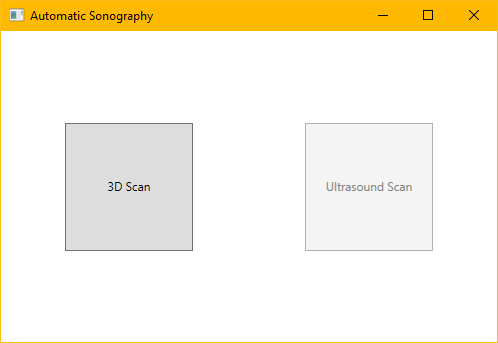
\includegraphics[width=0.5\textwidth]{figurer/d/GUIskitse/main_menu}
    \caption{3D Scan menu}
    \label{3Dscan}
\end{figure}

\begin{figure}[H]
    \centering
    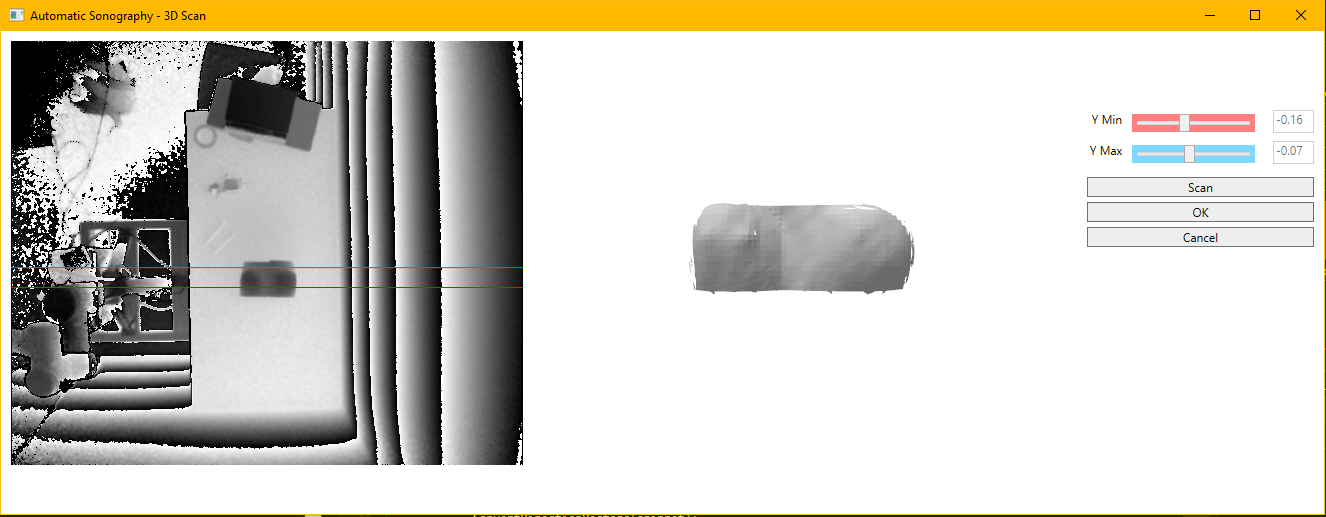
\includegraphics[width=0.5\textwidth]{figurer/d/GUIskitse/3d_scan}
    \caption{3D Scan menu}
    \label{3Dscan}
\end{figure}

\begin{figure}[H]
    \centering
    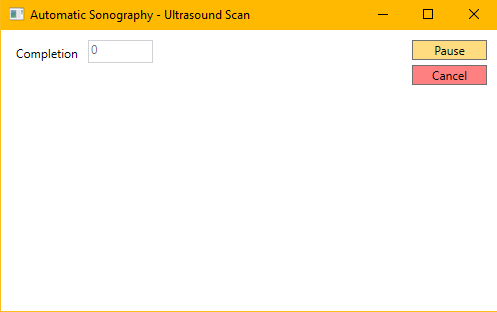
\includegraphics[width=0.5\textwidth]{figurer/d/GUIskitse/ultrasound_scan}
    \caption{Ultralydsscan menu}
    \label{Ultralydsscan}
\end{figure}